\part{Logging and Tracing}

\begin{frame}{Motivation}

    \begin{block}{No debugging of running microservice in production}
            \begin{itemize}
                \item by default debug port is closed (and \codealt{SSH access} is disabled) 
                \item applications must be SOX compliant, i.e. immutable
                \item multiple instances, hard to target specific instance
            \end{itemize}
    \end{block}

	\begin{block}{``I saw some error message two weeks ago``}
	    \begin{itemize}
            \item Do you know which code ran at that time?
            \item Can you identify the corresponding request?
            \item Can you locate the problem if it happened in a downstream service?
            \item Do you have the data necessary to understand/reproduce the error?
	    \end{itemize}
    \end{block}
\end{frame}

\begin{frame}{What should be logged?}
	\begin{description}
		\item[Basics] timestamp (UTC), thread, logger name, severity
		\item[Operational] traces (for important methods), errors, configuration, \ldots{}
		\item[Categories] useful for filtering: SQL, Authentication, Order, \ldots{}
		\item[Business] used features, purchases, response times (SLA?), \ldots{}
		\item[Security] login, denied access, privileged account actions, \ldots{}
		\item[Correlation] same ID in all messages for a request, propagate!
	\end{description}

    \vfill
    \visible<2->{
	    \centerline{\textbf{Brainstorm! Think about scenarios!}}
	}
\end{frame}

\begin{frame}{What should NOT be logged?}
    \begin{itemize}
        \item Passwords, credit card details, personal information, \ldots{}
        \item Confidential information
        \item Respect rules set up by regulations and legislations
        \item Log IDs instead of sensitive data\\(e.g. \textit{user ID} instead of \textit{name}, \textit{email}, \ldots)
        \item \textbf{Attention:} Sensitive data in REST URIs or stack traces
    \end{itemize}

    \vfill
    \colorlink{https://wiki.wdf.sap.corp/wiki/display/technology/Telemetry\#Telemetry-LegalQuestions\%3AWhatareweallowedtotrack\%3F}{Read also: What are we allowed to track?}
\end{frame}

\begin{frame}{Big Picture}
\centerline{
	\includeGraphicsLoggingBigPicture{width=0.9\textwidth}
}
\end{frame}

\begin{frame}[fragile]{Logging Library and SLF4J}{Simple Logging Facade for Java}
	\begin{block}{Logging Library}
	    \colorlink{https://github.com/SAP/cf-java-logging-support}{SAP Java Logging Support for Cloud Foundry}
	    \begin{itemize}
	        \item JSON formatting
	        \item Servlet Filter: logs performance data and more
	    \end{itemize}
    \end{block}

    SLF4J Implementations: \underline{Logback}, Log4J\,2, \ldots{}

    \vfill

    \begin{lstlisting}
import org.slf4j.*;
// ...
Logger logger = LoggerFactory.getLogger(Foo.class);
// request = ...
logger.info("incoming request: {}", request);
    \end{lstlisting}
\end{frame}

\begin{frame}[fragile]{Overview Log Levels}{... and when to use what?}
    The levels in descending order are:
    \begin{description}
        \item[error] for critical exceptions that need immediate attention
        \item[warn] for exceptions that do not trigger alerts, e.g. NotFound
        \item[info] for (API, REST) requests, used features
        \item[debug] for information helpful only when debugging, e.g. subtotals
        \item[trace] for very detailed information, e.g. parameter values
    \end{description}

    \vfill
    Typically only messages of severity \codealt{INFO} or higher are logged in production.
    \vfill
    \textbf{NOTE:} The application logging service will only permit a certain amount of logs per timeframe based on your \colorlink{https://go.sap.corp/logging}{plan}.
   \textbf{All logs exceeding this quota will be dropped!}
\end{frame}

\begin{frame}{Log Formatting}
\begin{block}{Output Format}
Human Readable, JSON, XML, \ldots
\end{block}

\begin{block}{Customization}
        \begin{itemize}
            \item date format (\codealt{2016-02-29 14:55:52}, \codealt{1441720072}, \ldots)
            \item package representation (\codealt{com.sap.foo.Bar}, \codealt{c.s.f.Bar}, \ldots)
            \item additional details (thread name, log level, \ldots)
        \end{itemize}
\end{block}
Examples:
{\footnotesize
\begin{itemize}
    \item \codealt{2016-02-29 14:55:52 INFO com.sap.foo.Bar:5 - incoming request: [source=10.1.2.3, uri=/some/where/23]}
    \item \codealt{1441720072 [INFO] [c.s.f.Bar] [663a1be8] [SomeThread] incoming request: [source=10.1.2.3, uri=/some/where/23]}
\end{itemize}
}
% PLAIN vs. JSON
% XML, different date formats, ...
\end{frame}

\begin{frame}{Exercise 12}
	\begin{figure}
		\includeGraphicsExerciseTwelve{width=0.7\textwidth}
	\end{figure}
	\colorlink{https://github.wdf.sap.corp/cc-java-dev/cc-coursematerial/blob/master/LoggingTracing/Exercise_12_Setup_Logger.md}{Exercise 12: Setup Logger}
\end{frame}

\begin{frame}[fragile]{Implementation Hints}
	\begin{itemize}
	\item Use \codealt{getClass()} to avoid copy-paste errors (in non-static context):
    \begin{lstlisting}
Logger logger = LoggerFactory.getLogger(getClass());
    \end{lstlisting}

    \begin{visibleenv}<2->
        \item Avoid String concatenation, use\\ \begin{lstlisting}
logger.trace("msg:{}", arg)
        \end{lstlisting} instead of \begin{lstlisting}
logger.trace("msg:" + arg)
        \end{lstlisting}
    \end{visibleenv}

    \begin{visibleenv}<3->
        \item Use \codealt{isXXXEnabled} for expensive constructs
        \begin{lstlisting}
if (logger.isDebugEnabled()) {
    Object argument = thisIsExpensive();
    logger.debug("msg:{}", argument);
}
        \end{lstlisting}
    \end{visibleenv}

    \visible<4->{
        \item \colorlink{http://www.slf4j.org/faq.html\#logging\_performance}{Further performance hints}
    }
	\end{itemize}
\end{frame}


\begin{frame}[fragile]{Correlation ID and MDC}{Mapped Diagnostic Context}
    \begin{block}{Correlation ID}
        \begin{itemize}
            \item correlates log messages of different microservices
            \item automatically added to MDC using servlet filter
            \item manually add to outgoing request headers
        \end{itemize}
    \end{block}

    \vfill

    Provide information in MDC - once per thread\ldots{}
    \begin{lstlisting}
MDC.put("endpoint", "something/" + id);
    \end{lstlisting}
    \ldots{}so that it is included in all messages of the same thread

    \begin{lstlisting}
logger.info("customer {} logged in", customer.getId());
// 1441720072 [INFO] [c.s.f.Bar] [endpoint=something/1234] customer 1234 logged in
logger.info("customer used feature");
// 1441720073 [INFO] [c.s.f.Bar] [endpoint=something/1234] customer used feature
    \end{lstlisting}

\end{frame}

% TODO: Marker?

\begin{frame}{Exercise 13}
\colorlink{https://github.wdf.sap.corp/cc-java-dev/cc-coursematerial/blob/master/LoggingTracing/Exercise_13_Use_SLF4J_Features.md}{Exercise 13: Use SLF4J Features}
\end{frame}

\begin{frame}[fragile]{Trace Methods with Aspect-Oriented Programming}
With Java Aspects (e.g. \codealt{AspectJ})\footnote{Aspects modularize cross-cutting concerns, applying logic that spans multiple objects} you can easily introduce trace logs 
\begin{itemize}
\item for every method execution
\item seeing what arguments it receives
\item what it returns 
\item and how much time every execution takes
\end{itemize}
\textbf{without changing code!}

\vfill
\colorlink{https://github.wdf.sap.corp/cc-java-dev/cc-coursematerial/blob/master/LoggingTracing/AOP.md}{Examples: Trace Aspects}
\end{frame}

\begin{frame}{Analyze Your Logs @CF}{ELK Stack}
\begin{itemize}
\item Logs are only useful if they can be analyzed 
\item Collect logs in single location $\rightarrow$ common format required
\item ELK stack: \textbf{E}lasticsearch + \textbf{L}ogstash + \textbf{K}ibana is a popular combination to store, search, and view log entries.
\item[] $\hookrightarrow$ provided at CF @ SAP CP
\end{itemize}
\vfill
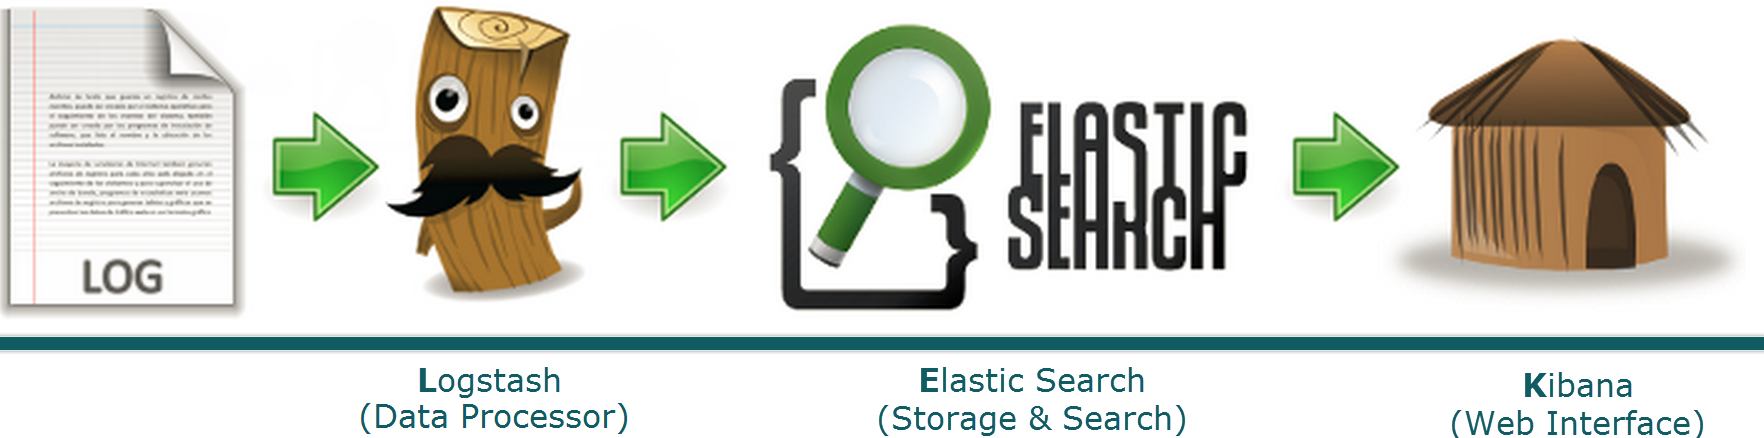
\includegraphics[width=\textwidth]{../LoggingTracing/images/ELK}
\end{frame}

\begin{frame}{Exercise 14}
\begin{figure}
		\includeGraphicsExerciseFifteen{width=0.7\textwidth}
	\end{figure}
\colorlink{https://github.wdf.sap.corp/cc-java-dev/cc-coursematerial/blob/master/LoggingTracing/Exercise_14_GettingStarted_With_ELK_Stack.md}{Exercise 14: Getting started with the ELK stack}
\end{frame}


\begin{frame}{Other Logging Services @ SAP CP CF}
For building Enterprise applications, application logs are not sufficient!
Apart from Application Logs , SCP CF offers the below services
\vfill
\begin{itemize}
  \item \textbf{Audit Log Service} (\colorlink{https://github.wdf.sap.corp/xs-audit-log/sap-cp-audit-log-service-docs/wiki}{Wiki})
     \begin{itemize}
	    \item \textbf{Audit Logs}: log audit relevant information (\colorlink{https://wiki.wdf.sap.corp/wiki/display/PSSEC/SEC-257}{SEC-257}, \colorlink{https://wiki.wdf.sap.corp/wiki/display/PSSEC/SEC-265}{SEC-265})) 
		\\that needs to be kept for a longer time period. 
		\\E.g. Who changed What data When [and How] [and Why].
        \item \textbf{Read Access Logs}: log access of sensitive information (\colorlink{https://wiki.wdf.sap.corp/wiki/display/PSSEC/SEC-254}{SEC-254})
		\\E.g. Access to health records, religious beliefs etc.
		\item \textbf{Security Logs} log \textbf{security events} (\colorlink{https://wiki.wdf.sap.corp/wiki/display/PSSEC/SEC-257}{SEC-215})
        \\E.g. Failed authorization checks, password change etc.
     \end{itemize}
  \item \textbf{Business Log Service} (\colorlink{https://jam4.sapjam.com/groups/d5rFGe6JlU5MM9zOJLlhiB/overview_page/ncmsQCfeIyozHxe9nWIrmh}{Jam Group})
     \begin{itemize}
        \item To be used to document \textbf{Business Flow} for later troubleshooting.
        \\E.g. Background tasks, Workflow etc.
     \end{itemize}
\end{itemize}
\vfill
Each of them offers \textbf{unique features}\\
You need to pick the right one depending on your use case!
\end{frame}